%%%%%%%%%%%%%%%%%%%%%%%%%%%%%%%%%%%%%%
\section{Estimation with gaussian distributions}
%%%%%%%%%%%%%%%%%%%%%%%%%%%%%%%%%%%%%%

In this section we will analyze the case of random variable estimation when the combined distribution of all the variables involved (variable to be estimated and observation variables) is a multidimensional Gaussian. This case is of special interest given the frequency with which these distributions usually appear in problems in the field of telecommunications and in other scenarios. In this case, it can be shown that all marginal distributions and all conditional distributions are also Gaussian. Specifically, given that $p_{S|{\bf X}} (s|{\bf x})$ is Gaussian, it can be understood that the fashion, the mean and the median of the distribution coincide, so $\hat{s}_{\text{MSE}} = \hat{s}_{\text{MAD}} = \hat{s}_{\text{MAP}}$ will be verified. Therefore, during this section we will focus our discussion on the calculation of the minimum quadratic mean error estimator. 

Besides, we will demonstrate that the MSE estimator and, consequently, the MAP and MAD estimators are linear, which will allow us to use the results shown in the previous section for minimum mean squared error estimators.


%%%%%%%%%%%%%%%%%%%%%%%%%%%%%%%%
\subsection{One dimensional case}

We will consider as a starting point a case with one-dimensional random variables with zero means, in which the joint distribution of $X$ and $S$ has the following form:

\begin{equation}
p_{S,X}(s,x) \sim G\left(\left[\begin{array}{c} 0 \\ 0 \end{array}\right],\left[\begin{array}{cc} v_S & \rho \\ \rho & v_X \end{array}\right]\right)
\end{equation}
where $\rho$ is the covariance between the two random variables.

From this joint distribution we can obtain any other distribution involving the variables $s$ and $x$; specifically, the posterior distribution of $S$ can be obtained as:

\begin{equation}
\begin{split}
p_{S|X}(s|x) & = \frac{p_{S,X}(s,x)}{p_X(x)} \\
& = \displaystyle\frac{\displaystyle\frac{1}{2\pi \sqrt{v_X v_S - \rho^2}}\exp\left[-\displaystyle\frac{1}{2(v_X v_S - \rho^2)}\left[\begin{array}{c} s \\ x \end{array}\right]^T\left[\begin{array}{cc} v_X & -\rho \\ -\rho & v_S \end{array}\right] \left[\begin{array}{c} s \\ x \end{array}\right]\right]}{\displaystyle\frac{1}{\sqrt{2\pi v_X}} \exp\left[-\displaystyle\frac{x^2}{2 v_X}\right]}
\end{split}
\end{equation}

where it has been necessary to calculate the inverse of the covariance matrix of $S$ and $X$, which is easy since the matrix has dimensions of $2 \times 2$.

Our goal for obtaining $\hat s_{\text{MSE}}$ is to calculate the mean of that distribution. However, a direct calculation by integrating your product with $s$ is quite complicated. However, given the joint Gaussian character of $S$ and $X$, we know that the posterior distribution of $S$ must necessarily be Gaussian, defined by its (unknown) parameters of mean and variance $m_{S|X}$ and $v_{S|X}$, respectively, allowing the above expression to be rewritten as:

\begin{multline}
\frac{1}{\sqrt{2\pi v_{S|X}}} \exp\left[ -\frac{(s - m_{S|X})^2}{2 v_{S|X}}\right] = \\ \displaystyle\frac{\displaystyle\frac{1}{2\pi \sqrt{v_X v_S - \rho^2}}\exp\left[-\displaystyle\frac{1}{2(v_X v_S - \rho^2)}\left[\begin{array}{c} s \\ x \end{array}\right]^T\left[\begin{array}{cc} v_X & -\rho \\ -\rho & v_S \end{array}\right] \left[\begin{array}{c} s \\ x \end{array}\right]\right]}{\displaystyle\frac{1}{\sqrt{2\pi v_X}} \exp\left[-\displaystyle\frac{x^2}{2 v_X}\right]}
\end{multline}
It is possible to break this equality down into two others associated with factors external to the exponentials and their arguments:

\begin{equation}
\label{ec:gauss_iguald1}
\frac{1}{\sqrt{2\pi v_{S|X}}} = \frac{\sqrt{2\pi v_X}}{{2\pi \sqrt{v_X v_S - \rho^2}}}
\end{equation}
\begin{equation}
\label{ec:gauss_iguald2}
\frac{(s - m_{S|X})^2}{v_{S|X}} = \displaystyle\frac{1}{v_X v_S - \rho^2}\left[\begin{array}{c} s \\ x \end{array}\right]^T\left[\begin{array}{cc} v_X & -\rho \\ -\rho & v_S \end{array}\right] \left[\begin{array}{c} s \\ x \end{array}\right] - \displaystyle\frac{x^2}{v_X}
\end{equation}
By operating the matrix terms, the second of these equals can be more simply rewritten as
\begin{equation}
\label{ec:gauss_iguald2bis}
\frac{(s - m_{S|X})^2}{v_{S|X}} = \displaystyle\frac{v_X s^2 + v_S x^2 - 2 \rho x s}{v_X v_S - \rho^2} - \displaystyle\frac{x^2}{v_X}
\end{equation}

Note that \eqref{ec:gauss_iguald2bis} assumes an equality between two polynomials in $s$ (and in $x$). Therefore, the coefficients of the independent, linear and quadratic terms in $s$ (i.e., which do not depend on $s$, or which multiply to $s$ and $s^2$) that appear on both sides of the equality must match. Therefore, and taking into account that $m_{S|X}$ does not depend on $s$, the following three equality must be verified:

\begin{equation}
\label{ec:gauss_iguald3}
\frac{m_{S|X}^2}{v_{S|X}} = \displaystyle\frac{v_S x^2}{v_X v_S - \rho^2} - \displaystyle\frac{x^2}{v_X}
\end{equation}
\begin{equation}
\label{ec:gauss_iguald4}
\frac{s\;m_{S|X}}{v_{S|X}} = \displaystyle\frac{\rho x s}{v_X v_S - \rho^2}
\end{equation}
\begin{equation}
\label{ec:gauss_iguald5}
\frac{s^2}{v_{S|X}} = \displaystyle\frac{v_X s^2}{v_X v_S - \rho^2}
\end{equation}
For the calculation of the posterior mean, it is convenient solving \eqref{ec:gauss_iguald4} for $m_{S|X}$ as
\begin{equation}
\label{ec:msx_parcial}
m_{S|X} = \frac{v_{S|X} \rho x}{v_X v_S - \rho^2}
\end{equation}
Finally, the value of the posterior variance can easily be extracted from \eqref{ec:gauss_iguald1} or \eqref{ec:gauss_iguald5} as
\begin{equation}
v_{S|X} = \frac{v_X v_S - \rho^2}{v_X}
\end{equation}
Replacing this value in \eqref{ec:msx_parcial} gives the expression that determines the minimum quadratic mean error estimator.
\begin{framed}
\begin{equation}
\label{ec_estimador_caso_gaussiano_final}
\hat s_{\text{MSE}} = m_{S|X} = \frac{\rho}{v_X} x
\end{equation}
\end{framed}
As can be seen, the estimator obtained is \underline{linear}.

%%%%%%%%%%%%%%%%
\begin{exercise}
Generalize the above result for the case where the variables $S$ and $X$ have (non-zero) means $m_S$ and $m_X$, respectively. Demonstrate that in such a case, the estimator is
\begin{equation}
\hat s_{\text{MSE}} = m_S + \frac{\rho}{v_X} (x - m_X)
\end{equation}
\end{exercise}
%%%%%%%%%%%%%%

%%%%%%%%%%%%%%%
\begin{example}[Estimation of a Gaussian signal contaminated by Gaussian noise]
\label{ex:senialenruido}

In this example we will consider the case in which the observation is obtained as the sum of the signal to be estimated and a noise component independent of the signal: $X = S + R$. Both the signal and the noise present Gaussian distributions of zero means and variances $v_S$ and $v_R$, respectively.

Figure \eqref{fig:estimacion_caso_gauss} represents the situation described for a case with $v_S < v_R$.
\begin{figure}[htb]
  \begin{center}
  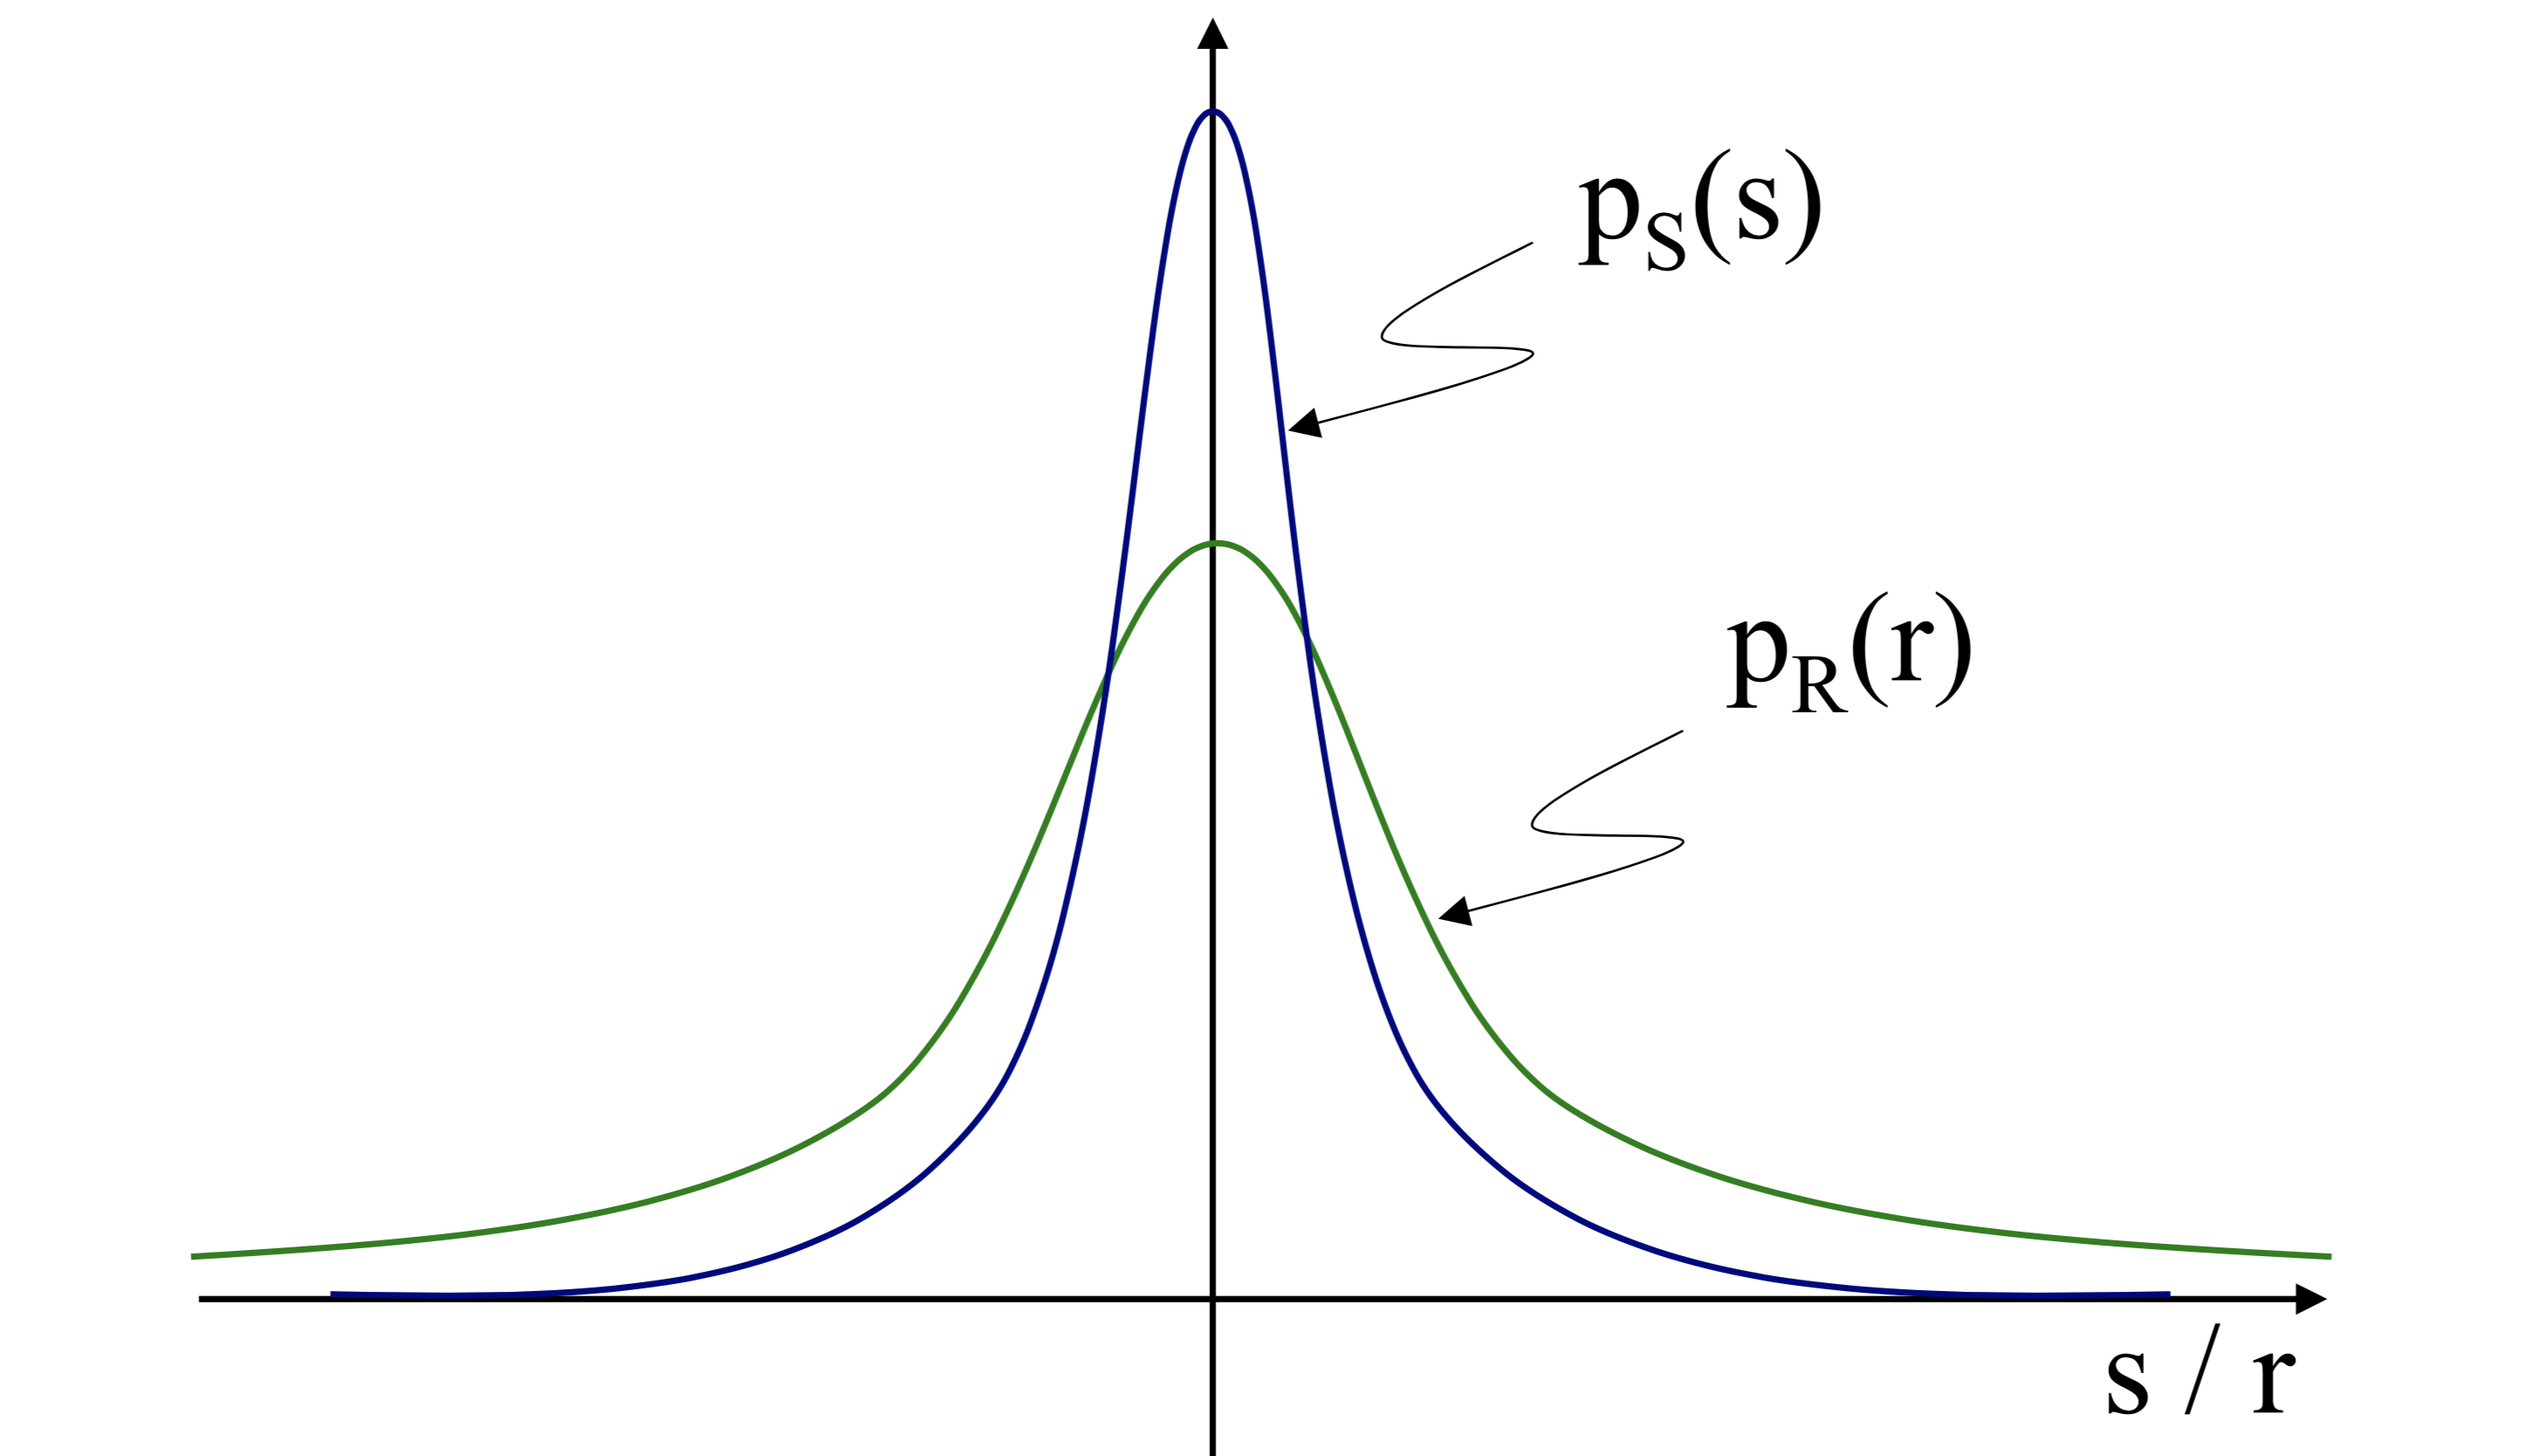
\includegraphics[width=10cm]{Figures//estimacion_caso_gauss.png}
    \caption{Estimation of Gaussian random variable $S$ contaminated by Gaussian noise $R$.}
    \label{fig:estimacion_caso_gauss}
  \end{center}
\end{figure}
\end{example}\vspace{0.4cm}
%%%%%%%%%%%%%

According to \eqref{ec_estimador_caso_gaussiano_final}, for the resolution of the problem we must find the variance of $X$ and the covariance between $S$ and $X$ ($\rho$). The variance $v_X$ is obtained simply as the sum of $v_S$ and $v_R$ because both are independent variables. For the covariance calculation we can proceed as follows:

\begin{equation}
\rho = \mathbb{E} \{(X-m_X)(S-m_S)\} = \mathbb{E} \{X\;S\} = \mathbb{E} \{(S + R) S\} = \mathbb{E} \{S^2\} + \mathbb{E} \{S\;R\} = v_S
\end{equation}

where independence of $S$ and $R$ has been used, and the fact that all variables (including $X$) have zero means.

Replacing these results in \eqref{ec_estimador_caso_gaussiano_final} we get

\begin{equation}
\hat s_{\text{MSE}} = \frac{v_S}{v_S + v_R} x
\end{equation}

This result can be interpreted quite intuitively: when the variance of the noise is much lower than that of the signal (high Signal to Noise Ratio (SNR), $v_S \gg v_R$) you have to  $\hat s_{\text{MSE}} \to x$, which makes sense since the effect of the noise component in this case is not very significant; on the contrary, when the SNR is very low ($v_S \ll v_R$), the observation barely provides information about the $S$ value in each experiment, so the estimator keeps the mean value of the signal component, $\hat s_{\text{MSE}} \to 0$.


%%%%%%%%%%%%%%%%%%%%%%%%%%%%%%%%%%%%%%%%%%%%%%%%%%
\subsection{Case with multidimensional variables}

{In a general multidimensional case, ${\bf S}$ and ${\bf X}$ can be random vectors of dimensions $N$ and $M$, respectively, with joint Gaussian distribution.
\begin{equation}
p_{{\bf S},{\bf X}}({\bf s},{\bf x}) 
   \sim G\left(\left[\begin{array}{c} {\bf m_S} \\ {\bf m_X} \end{array}\right],
               \left[\begin{array}{cc} {\bf V_S}          & {\bf V_{SX}}   \\ 
                                       {\bf V}_{\bf SX}^T & {\bf V_{X}}   
                     \end{array}\right]\right)
\end{equation}
being ${\bf m_S}$ and ${\bf m_X}$ the means of $ {\bf S}$ and $ {\bf X}$, respectively, ${\bf V_S}$ and ${\bf V_X}$ the covariance matrix of ${\bf S}$ and  ${\bf X}$, respectively, and ${\bf V_{SX}}$ the matrix of crossed covariances of ${\bf S}$ and ${\bf X}$, that is,
\begin{equation}
{\bf V_S} = \mathbb{E}\{({\bf S}-{\bf m_S})({\bf S}-{\bf m_S})^T\} \\
\end{equation}
\begin{equation}
{\bf V_X} = \mathbb{E}\{({\bf X}-{\bf m_X})({\bf X}-{\bf m_X})^T\}
\end{equation}
\begin{equation}
{\bf V_{SX}} = \mathbb{E}\{({\bf S}-{\bf m_S})({\bf X}-{\bf m_X})^T\}
\end{equation}
%La expresión general de la densidad de probabilidad es, por tanto
%\begin{align}
%p_{{\bf S},{\bf X}}({\bf s},{\bf x}) 
%   & = \frac{1}
%            {(2\pi)^{(M+N)/2} 
%             \left|\left[\begin{array}{cc} 
%                          {\bf V_S}    & {\bf V_{SX}}   \\ 
%                          {\bf V}_{\bf SX}^T & {\bf V_{X}} 
%                         \end{array}\right]
%             \right|^{1/2}} \times \nonumber\\
%    &  \times\exp\left[-\frac{1}{2}
%                  \left[\begin{array}{c} {\bf s}-{\bf m_S} \\ {\bf x}-{\bf m_X} \end{array}\right]^T                       
%                  \left[\begin{array}{cc} 
%                           {\bf V_S}          & {\bf V_{SX}} \\ 
%                           {\bf V}_{\bf SX}^T & {\bf V_{X}} 
%                        \end{array}\right]^{-1}
%                  \left[\begin{array}{c} {\bf s} \\ {\bf x} \end{array}\right]
%       \right]
%\end{align}
%La distribución a posteriori de $S$ se puede obtener como:
%\begin{align}
%p_{{\bf S}|{\bf X}}({\bf s}|{\bf x}) 
%   & = \frac{p_{{\bf S},{\bf X}}(s,x)}{p_{\bf X}(x)} \nonumber\\
%   & = \frac{(2\pi)^{M/2}|{\bf V}_{\bf X}|^{1/2}}
%            {(2\pi)^{(M+N)/2} 
%             \left| \left[\begin{array}{cc} 
%                             {\bf V_S}    & {\bf V_{SX}}   \\ 
%                           {\bf V}_{\bf SX}^T & {\bf V_{X}} 
%                    \end{array}\right]
%                    \right|^{1/2}} \times \nonumber\\
%    &  \times\exp\left[-\frac{1}{2}
%                  \left[\begin{array}{c} {\bf s} \\ {\bf x} \end{array}\right]^T                       
%                  \left[\begin{array}{cc} 
%                           {\bf V_S}          & {\bf V_{SX}} \\ 
%                           {\bf V}_{\bf SX}^T & {\bf V_{X}} 
%                        \end{array}\right]^{-1}
%                  \left[\begin{array}{c} {\bf s} \\ {\bf x} \end{array}\right]
%                 -\frac{1}{2} {\bf x}^T{\bf V_X}^{-1}{\bf x} \right]
%\end{align}

The calculation of the posterior distribution of ${\bf S}$ given ${\bf X}$ is more complex than in the one-dimensional case, but it follows a similar procedure, which we will omit here. It can be shown that the posterior distribution is gaussian with mean

\begin{align}
{\bf m}_{{\bf S}|{\bf X}} 
      = {\bf m}_{\bf S} + {\bf V}_{\bf SX}{\bf V_X}^{-1}({\bf x}-{\bf m}_{\bf X}) 
\label{Est:sMMSEgaussMN}
\end{align}
\noindent and covariance
\begin{align}
{\bf V}_{{\bf S}|{\bf X}} 
      = {\bf V_S}- {\bf V}_{\bf SX}{\bf V_X}^{-1}{\bf V}_{\bf SX}^T
\end{align}
Since the MMSE estimator of ${\bf S}$ given ${\bf X}$ is precisely the posterior mean, we can write

\begin{framed}
\begin{align}
\hat{\bf s}_{\text{MSE}} = {\bf m}_{\bf S} + {\bf V}_{\bf SX}{\bf V_X}^{-1}({\bf x}-{\bf m}_{\bf X}) 
\label{Est:sMMSEgaussGral}
\end{align}
\end{framed}
This estimator expression is simplified when ${\bf S}$ and ${\bf X}$ have zero means, resulting in
\begin{align}
\hat{\bf s}_{\text{MSE}} = {\bf m}_{{\bf S}|{\bf X}} 
      = {\bf V}_{\bf SX}{\bf V_X}^{-1}{\bf x} 
      \label{Est:sMMSEgaussMN0}
\end{align}}
%Partiendo de \eqref{Est:sMMSEgaussMN0} pueden obtenerse diversos casos particulares de interés en aplicaciones prácticas del procesado de señales. Algunos de ellos se analizan en el Apéndice \ref{Sec:Est:CasosGauss}.


\subsection{Linear estimation and Gaussian estimation}

Regrouping the terms of \eqref{Est:sMMSEgaussGral}, we can express $\hat{\bf s}_{\text{MSE}}$ as:
\begin{framed}
\begin{align}
\hat{\bf s}_{\text{MSE}} = ({\bf m}_{\bf S} - {\bf V}_{\bf SX}{\bf V_X}^{-1}{\bf m}_{\bf X} )+ {\bf V}_{\bf SX}{\bf V_X}^{-1}{\bf x} 
\end{align}
\end{framed}
and identifying these terms with the coefficients of a linear estimator, we get
\begin{align} 
{\bf w}^T =  {\bf V}_{\bf SX}{\bf V_X}^{-1}
\end{align}
\begin{align} 
w_0 = {\bf m}_{\bf S} - {\bf w}^T {\bf m}_{\bf X}
\end{align}
These expressions coincides with the alternatives solution of the linear estimation of mean squared error (equations \ref{ec:solucionw0} and  \ref{ec:solucionw}).This is not surprising: since the unrestricted MSE estimator in the Gaussian case is linear, the best linear estimator must match the one obtained for the Gaussian case.

%Obsérvese, por último, que \eqref{ec:solucionw} asume que {${\bf V}_{\bf X}$} es una matriz no singular. La invertibilidad de {${\bf V}_{\bf X}$} implica que ninguna componente de ${\bf X}$ puede obtenerse como combinación lineal del resto de componentes. Cuando esto no es así, puede comprobarse que la solución al problema de minimización no es única, y por lo tanto conviene eliminar las variables redundantes antes de proceder al diseño del estimador.

